\chapter{\IfLanguageName{dutch}{Stand van zaken}{State of the art}}%
\label{ch:stand-van-zaken}

% Tip: Begin elk hoofdstuk met een paragraaf inleiding die beschrijft hoe
% dit hoofdstuk past binnen het geheel van de bachelorproef. Geef in het
% bijzonder aan wat de link is met het vorige en volgende hoofdstuk.

% Pas na deze inleidende paragraaf komt de eerste sectiehoofding.

%Dit hoofdstuk bevat je literatuurstudie. De inhoud gaat verder op de inleiding, maar zal het onderwerp van de bachelorproef *diepgaand* uitspitten. De bedoeling is dat de lezer na lezing van dit hoofdstuk helemaal op de hoogte is van de huidige stand van zaken (state-of-the-art) in het onderzoeksdomein. Iemand die niet vertrouwd is met het onderwerp, weet nu voldoende om de rest van het verhaal te kunnen volgen, zonder dat die er nog andere informatie moet over opzoeken \autocite{Pollefliet2011}.

%Je verwijst bij elke bewering die je doet, vakterm die je introduceert, enz.\ naar je bronnen. In \LaTeX{} kan dat met het commando \texttt{$\backslash${textcite\{\}}} of \texttt{$\backslash${autocite\{\}}}. Als argument van het commando geef je de ``sleutel'' van een ``record'' in een bibliografische databank in het Bib\LaTeX{}-formaat (een tekstbestand). Als je expliciet naar de auteur verwijst in de zin (narratieve referentie), gebruik je \texttt{$\backslash${}textcite\{\}}. Soms is de auteursnaam niet expliciet een onderdeel van de zin, dan gebruik je \texttt{$\backslash${}autocite\{\}} (referentie tussen haakjes). Dit gebruik je bv.~bij een citaat, of om in het bijschrift van een overgenomen afbeelding, broncode, tabel, enz. te verwijzen naar de bron. In de volgende paragraaf een voorbeeld van elk.

%\textcite{Knuth1998} schreef een van de standaardwerken over sorteer- en zoekalgoritmen. Experten zijn het erover eens dat cloud computing een interessante opportuniteit vormen, zowel voor gebruikers als voor dienstverleners op vlak van informatietechnologie~\autocite{Creeger2009}.

%Let er ook op: het \texttt{cite}-commando voor de punt, dus binnen de zin. Je verwijst meteen naar een bron in de eerste zin die erop gebaseerd is, dus niet pas op het einde van een paragraaf.

%\lipsum[7-20]
% TODO: Inleiding stand van zaken
% TODO: Omzetten in subsection IP
\acrfull{ip} is het fundament van elk gestructureerd, goed functionerend en veilig netwerk. Het geeft de mogelijkheid efficiënt gegevens te routeren, netwerken te verdelen in meer beheersbare eenheden, toegang te beperken tot gevoelige data of systemen, services te identificeren en het oplossen van netwerkproblemen \autocite{Postel1981}. Dit hoofdstuk legt uit wat \acrfull{dns} en \acrfull{dhcp} is, waarom \acrshort{ipam} helpt bij het beheren van \acrshort{ip} netwerken en waarom \acrshort{http} nodig is om te communiceren met EIP. 

% TODO: Korte uitleg subnet en VLAN

\subsection{DNS}
\textcite{Mockapetris1987} schrijft dat \acrshort{dns} een systeem is dat \textit{resource records} gebruikt om onder andere vertalingen te voorzien tussen domeinnamen en \acrshort{ip}-adressen. Als voorbeeld kan je via de browser naar google surfen via het \acrshort{ip}-adres \textit{142.251.36.35} of via domeinnaam \textit{www.google.be}.

Zoals beschreven door \textcite{Mockapetris1987} voorziet \acrshort{dns} meerdere types resource records die netwerkbeheerders kunnen meegeven: 
\begin{itemize}
    % TODO beschrijven wat een resource record is
    \item \textbf{A}: Dit resource record beschrijft een host adres. 
    Vb. \textit{”server1.voorbeeld.com. IN A 192.168.1.1”} maakt de vertaling zodat het toestel met de domeinnaam \textit{server1.voorbeeld.com} bereikbaar is zowel via het \acrshort{ip}-adres \textit{192.168.1.1} als via de domeinnaam. 
    \item \textbf{CNAME}: Dit resource record beschrijft de canonieke naam van een host, het wordt gebruikt om een alias of subdomein naar het hoofddomein door te verwijzen. Vb. \textit{"www.voorbeeld.com. IN CNAME server1.voorbeeld.com"} zorgt dat server1 ook bereikbaar is via "\textit{www.voorbeeld.com}".
    \item \textbf{MX}: Dit resource record is een \textit{mail exchange} record en wordt gebruikt om aan te geven welke mailservers verantwoordelijk zijn voor het ontvangen van mails binnen een domein. vb. \textit{"voorbeeld.com. IN MX 10 mailserver.voorbeeld.com"} geeft de \acrshort{dns} server mee welke server de mailserver is.
    \item \textbf{NS}: Dit resource record is een \textit{name server} record, het beschrijft welke \acrshort{dns}-servers verantwoordelijk zijn voor het beheren van \acrshort{dns}-informatie voor een domein. Vb. \textit{"voorbeeld.com. IN NS dns1.voorbeeld.com"} verwijst naar \textit{dns1} als \acrshort{dns}-server voor het domein “\textit{voorbeeld.com}”.
    \item \textbf{PTR}: Dit resource record is een \textit{Pointer} record, het wordt gebruikt om via \acrshort{ip} een vertaling te vragen aan de \acrshort{dns}-server in plaats van via de naam.
    \item \textbf{SOA}: Dit resource record is een \textit{Start of Authority} record die belangrijke informatie bevat over de zone, zoals welke de primaire \acrshort{dns}-server, contactpersonen, etc. zijn.
\end{itemize}

\subsection{DHCP}
Dit protocol voorziet een framework voor het doorgeven van configuratie-informatie naar hosts (lees: computers) op het netwerk . Zo kan een computer bijvoorbeeld een \acrshort{ip}-adres ontvangen waarmee die kan communiceren binnen het netwerk waarop die is aangesloten \autocite{Droms1997}.

\acrshort{ip}-netwerken worden door netwerkbeheerders op een logische manier opgesplitst in subnetwerken. Hierbij worden de beschikbare \acrshort{ip}-adressen verdeeld in subnetwerken (subnet). Toestellen binnen subnet A zullen elkaar kunnen bereiken terwijl een toestel in een subnet B zonder de nodige routering geen verbinding zal kunnen maken met de toestellen in subnet A.

Voor \acrshort{dhcp} zullen netwerkbeheerders subnets (of pools van \acrshort{ip}-adressen) aanbieden aan de \acrshort{dhcp}-server. Die zal gebruik maken van deze pools door (onder andere) \acrshort{ip}-adressen uit te delen aan toestellen die verbinden op het netwerk en daarbij de \acrshort{dhcp}-server laten weten dat ze nog geen \acrshort{ip}-adres hebben.

\textcite{Droms1997} schrijft dat \acrshort{dhcp} drie mechanismes gebruikt voor het uitdelen van \acrshort{ip}-adressen:
\begin{itemize}
    \item \textbf{Automatisch}: Permanent toewijzen van een \acrshort{ip}-adres.
    \item \textbf{Dynamisch}: \acrshort{ip}-adres voor een bepaalde tijd toewijzen.
    \item \textbf{Manueel}: Een (door de netwerkbeheerder) vooraf bepaald \acrshort{ip}-adres toewijzen, in vakjargon noemt met dit een \acrshort{ip}-reservatie.
\end{itemize}

\subsection{IPAM}
Naast de vele uitdagingen die zowel \acrshort{dns} als \acrshort{dhcp} met zich meebrengen, is het beheren van de beschikbare IP-adressen een belangrijk facet in het takenpakket van de netwerkbeheerder. \textcolor{purple}{Een slecht beheerd netwerk kan leiden tot \acrshort{ip}-conflicten waarbij meerdere apparaten hetzelfde \acrshort{ip}-adres gebruiken, wat op zijn beurt dan weer kan leiden tot netwerkstoringen en onvoorspelbaar gedrag van apparaten. Daarnaast zou men ook weinig tot geen overzicht hebben van de beschikbare \acrshort{ip}-adressen en subnetten in het netwerk waardoor het moeilijker is om de beschikbare adressen te beheren en potentiële conflicten te identificeren.}

\subsection{DNS, DHCP en IPAM} % TODO: referentie fontein troubleshooten want crash
\textcolor{purple}{De integratie van \acrshort{dns}, \acrshort{dhcp} en \acrshort{ipam} in een enkel systeem wordt vaak aangeduid als \acrfull{ddi}. \acrshort{ddi} biedt een benadering voor het beheren van de essentiële netwerkelementen die nodig zijn voor een goed functionerende infrastructuur. Door DNS, DHCP en IPAM te combineren, kunnen organisaties profiteren van een geïntegreerde aanpak voor het beheer van hun netwerkmiddelen, waardoor efficiëntie en consistentie worden bevorderd. Zoals beschreven door \textcolor{red}{fontein2023} leggen \acrshort{ddi}-applicaties doorgaans de focus voornamelijk op \acrshort{ipam}. Het zijn toepassingen die de beschikbare \acrshort{IP}-adressen en subnetten op een gestructureerde, overzichtelijke manier weergeven. Doorgaans is \acrshort{ddi} geïntegreerd met de \acrshort{dns}- en \acrshort{dhcp}-servers waardoor men deze componenten vanuit een centrale plek kunnen beheren. Er zijn meerdere \acrshort{ddi}-softwarepakketten ter beschikking die aangeboden worden door bedrijven zoals Solarwinds, Infoblox, en EfficientIP. Universiteit Gent heeft ervoor gekozen om EfficientIP aan te schaffen dus deze bachelorproef zal hier gebruik van maken voor het automatisch beheren van het netwerk.}


\subsection{Huidige werking Universiteit Gent}
\textcolor{purple}{Bij de aanvang van de bachelorproef is het netwerk van Universiteit Gent nog volledig beheert via subnetbestanden. Binnen het netwerkteam van UGent werd een standaard bepaald en toegepast voor het nummeren en klasseren van subnetten, de zogenaamde ARWA-standaard (naar oud-werknemer ARsene WAuters). Dankzij scripts worden deze subnetbestanden uitgelezen en wordt alle nodige informatie doorgegeven aan o.a. de \acrshort{dns}- en \acrshort{dhcp}-servers.}

\subsubsection{Subnetbestanden}
\label{subnetbestanden}
\textcolor{purple}{Op basis van ARWA-standaard krijgt elk subnetbestand een naam: “subnet” + “subnet klasse (A/B/C/D/G/I/N/P/T/V/W)” + “laatste 2 octetten van het netwerkadres”, zo stellen bijvoorbeeld het subnetbestand “subnetB147.000” het subnet 157.193.147.0/24 voor en subnetbestand “subnetB050.128” het subnet 157.193.50.128/25. Deze ongecrypteerde tekstbestanden stellen elk een deel of een volledig subnet voor. Indien een subnet meer dan 254 beschikbare \acrshort{ip}-adressen bevat zullen er meerdere, opeenvolgende, subnetbestanden gebruikt worden.}
\textcolor{purple}{
\begin{itemize}
    % TODO: Nakijken waarvoor OS key staat in host
    \item Header: Elk bestand begint met een “header” waarin belangrijke metadata beschreven staat over het netwerk: subnet klasse, nummer, naam, beschrijving, subnet masker, default gateway, DNS-servers, opties of DHCP, DNS, dot1x en security actief staan, datum van aanmaken, plaatsen waar het subnet actief is (via FI-codes), commentaar, en eventueel nog ACL-lijnen om extra toegang te voorzien aan het netwerk. Zie afbeelding \ref{fig:header}
    \item Hosts: Afhankelijk van de grootte van het subnet kunnen er tot 254 hosts beschreven staan in het bestand. Elke host, of die nu reeds bezet is of niet, staat beschreven in het subnetbestand. Hierbij krijg je dan via een key-value formaat, een opsomming van alle informatie: “N: hostnummer”, “H: hostnaam”, “E1: \acrshort{mac}" en eventueel “E2: extra \acrshort{mac}”, “T: beschrijving toestel”, “M: optie om veel mails te mogen versturen (voor bv. kopieerautomaten)”, “CS: type host, client of server”, “BO: Boot options (pad/naar/bootoption@server)”, “OS:  \textcolor{red}{???}”, ”P: en P#: locatie waar het toestel is aangesloten op het netwerk”, “CO: commentaar netwerkadmin”, ”V1-5: vakgroep universiteit + gegevens van het hoofd van de vakgroep”, “C1-5: gegevens van host contactpersoon”, “DC: datum van aanmaken registratie” en “DM: datum laatste wijziging”, optioneel kan er ook nog informatie bij geplaatst worden voor \acrshort{dns} A en CNAME resource records “AA: en CA:”, het openzetten van de beveiliging richting de host “S: en SI:” en ook extra mailinformatie “MD:”. Op de optionele informatie na staat deze informatie steeds voor elke host in het bestand. Indien een host \acrshort{IP} nog vrij is en ter beschikking staat voor een manuele reservatie dan zal dit worden weergegeven door een de opsomming van alle sleutelwaarden, met telkens een lege waarde. Afbeelding a van figuur \ref{fig:host} toont een \acrshort{ip} registratie voor host \textit{demonstratietoestel}, afbeelding b geeft weer hoe een lege host is beschreven.
\end{itemize}
}

\begin{figure}[H]
    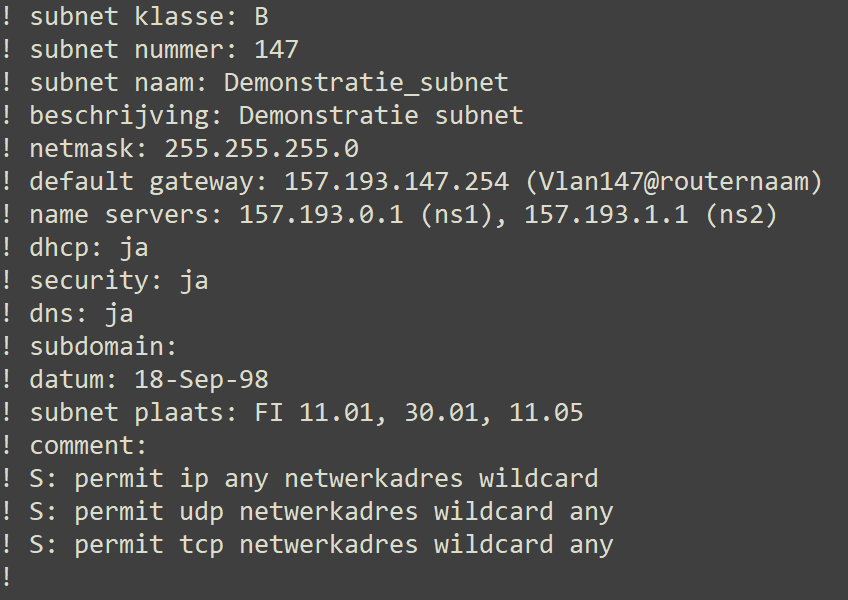
\includegraphics[height=7cm]{header.png}
    \caption{header}
    \label{fig:header}
\end{figure}

\begin{figure}[H]
    \subfloat[IP reservatie voor het eerste adres in het subnet]{%
        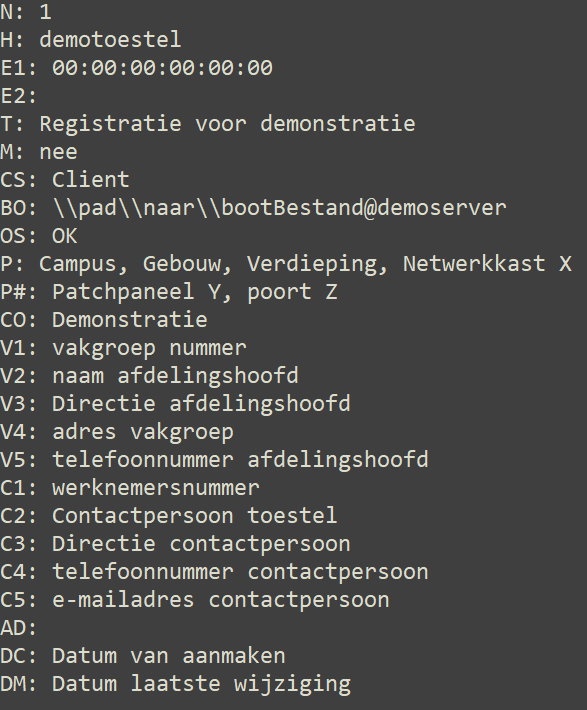
\includegraphics[height=0.4\textheight]{host.png}}
    \hspace*{\fill}
    \subfloat[Derde adres in het subnet is vrij om in te nemen]{%
        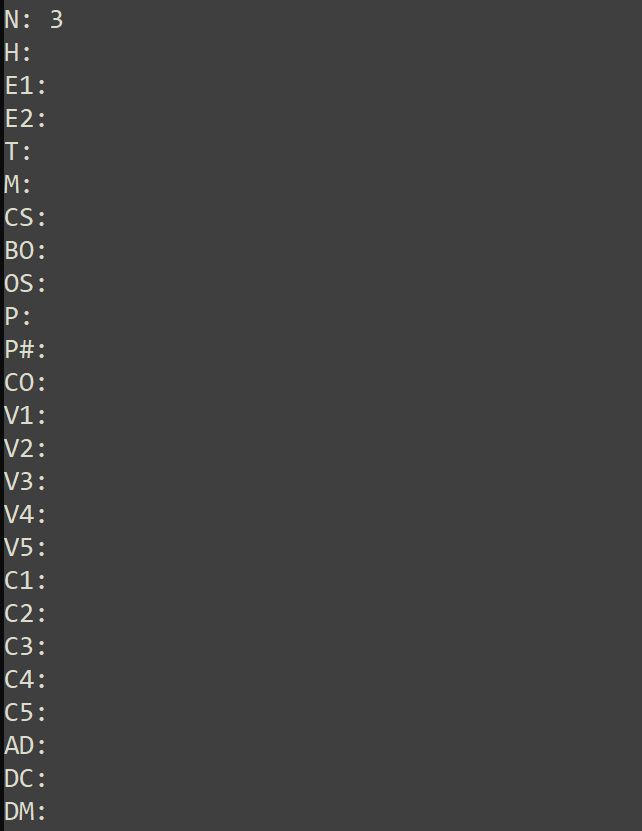
\includegraphics[height=0.4\textheight]{legeHost.png}}
    \caption{IP reservatie en lege host entry in subnetbestand}
    \label{fig:host}
\end{figure}



%\begin{figure}[h!]
%    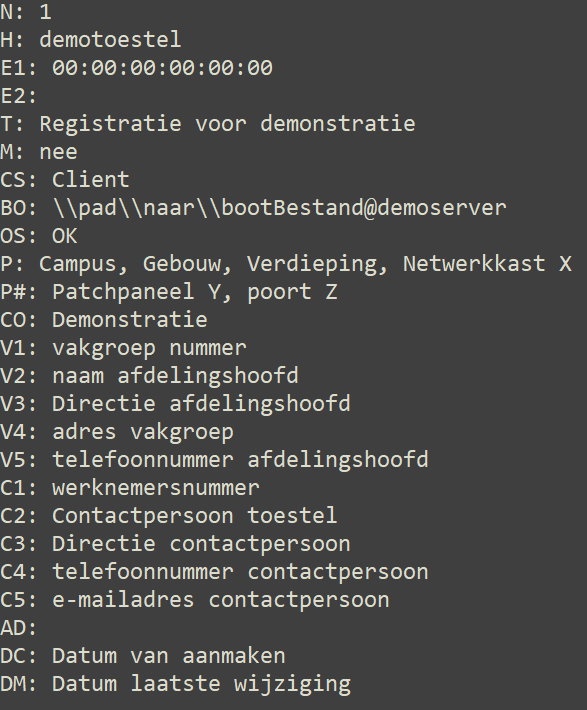
\includegraphics[scale=1.7]{host.png}
%    \caption{host}
%    \label{fig:host}
%\end{figure}
%\begin{figure}[h!]
%    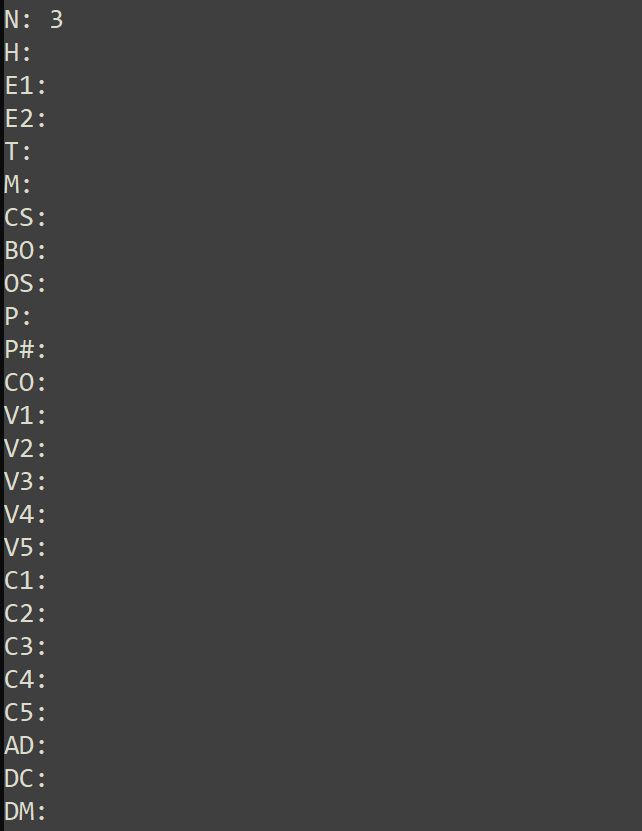
\includegraphics[scale=1.7]{legeHost.png}
%    \caption{lege Host}
%    \label{fig:legeHost}
%\end{figure}

\subsubsection{Procedure IP registratie voor gebruikers}
\textcolor{purple}{Via de interne webpagina www.netadmin.ugent.be kunnen werknemers van Universiteit Gent zowel nieuwe IP reservaties aanvragen, als bestaande IP reservaties raadplegen, wijzigen of verwijderen. Bij een nieuwe aanvraag kan men naast de basis info, ook de optionele parameters voor een host meegeven zoals beschreven in sectie \ref{subnetbestanden}. Bij wijzigingen kan men alle info van de registratie wijzigen, zo kan men info in de reservatie toevoegen, verwijderen of wijzigen. Het verplaatsen van een host van een subnet naar een ander is eveneens mogelijk, echter dient men dit door te geven aan de netwerkbeheerder via het opmerkingen-veld. In figuur \ref{fig:netadmin} zijn de formulieren van deze website weergegeven met data voor demonstratiedoeleinden.
}
\clearpage
\begin{figure*}[h!]
    \centering
    \begin{subfigure}[b]{0.475\textwidth}
        \centering
        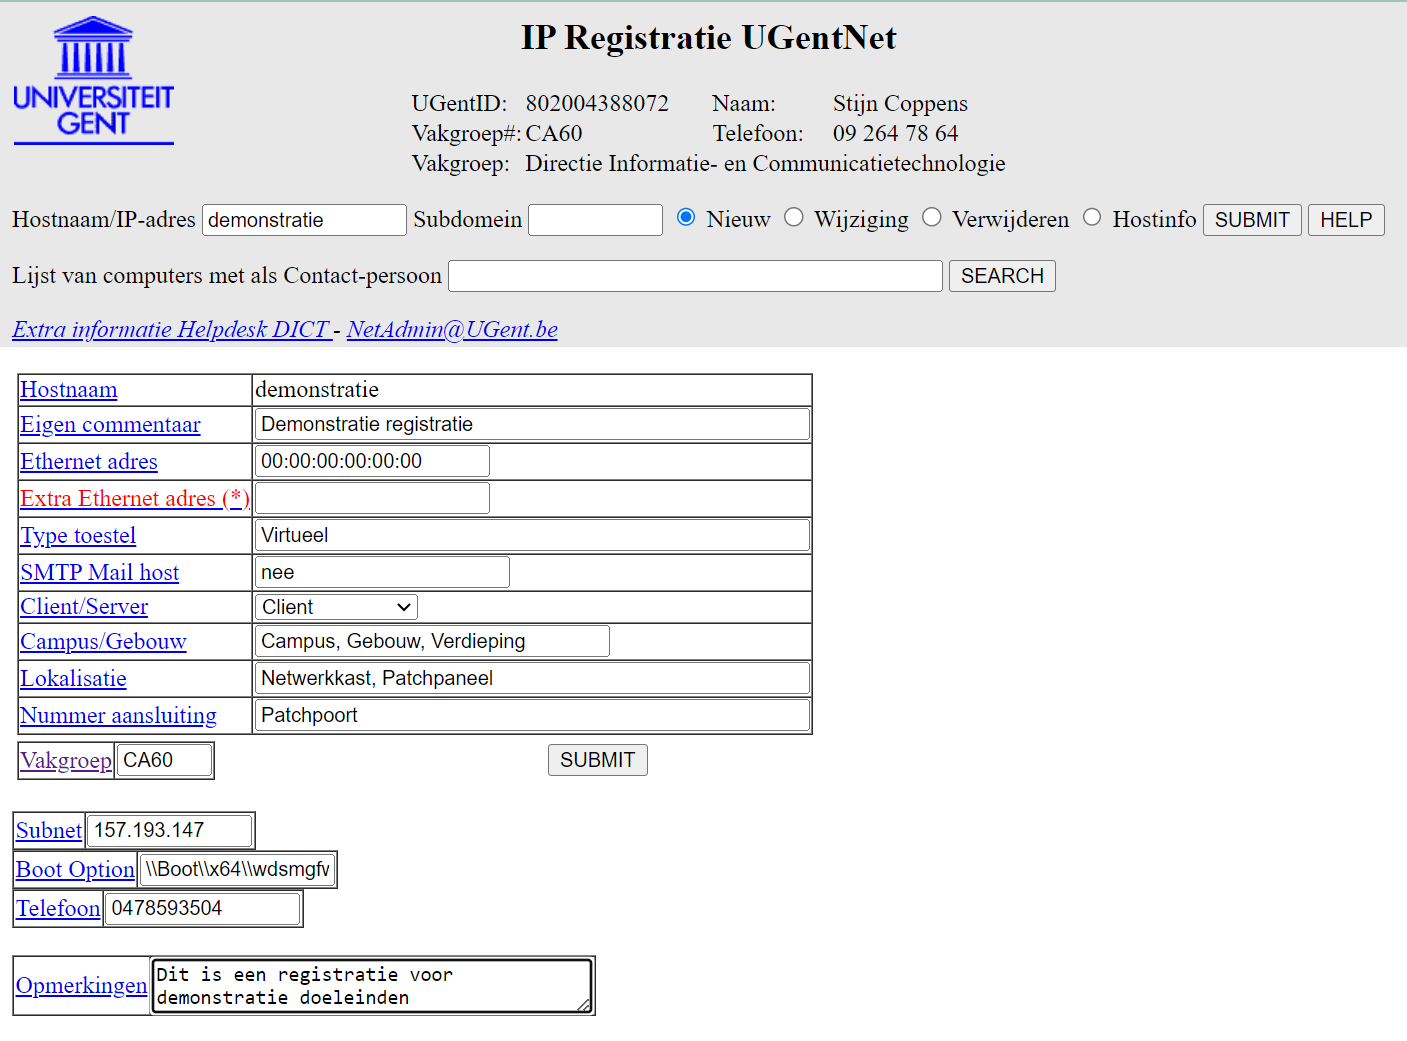
\includegraphics[width=\textwidth]{voorbeeldNieuweRegistratieNetadmin.png}
        \caption{Formulier nieuwe IP-registratie}
        \label{fig:formNieuwReg}
    \end{subfigure}%
    \hfill
    \begin{subfigure}[b]{0.475\textwidth}
        \centering
        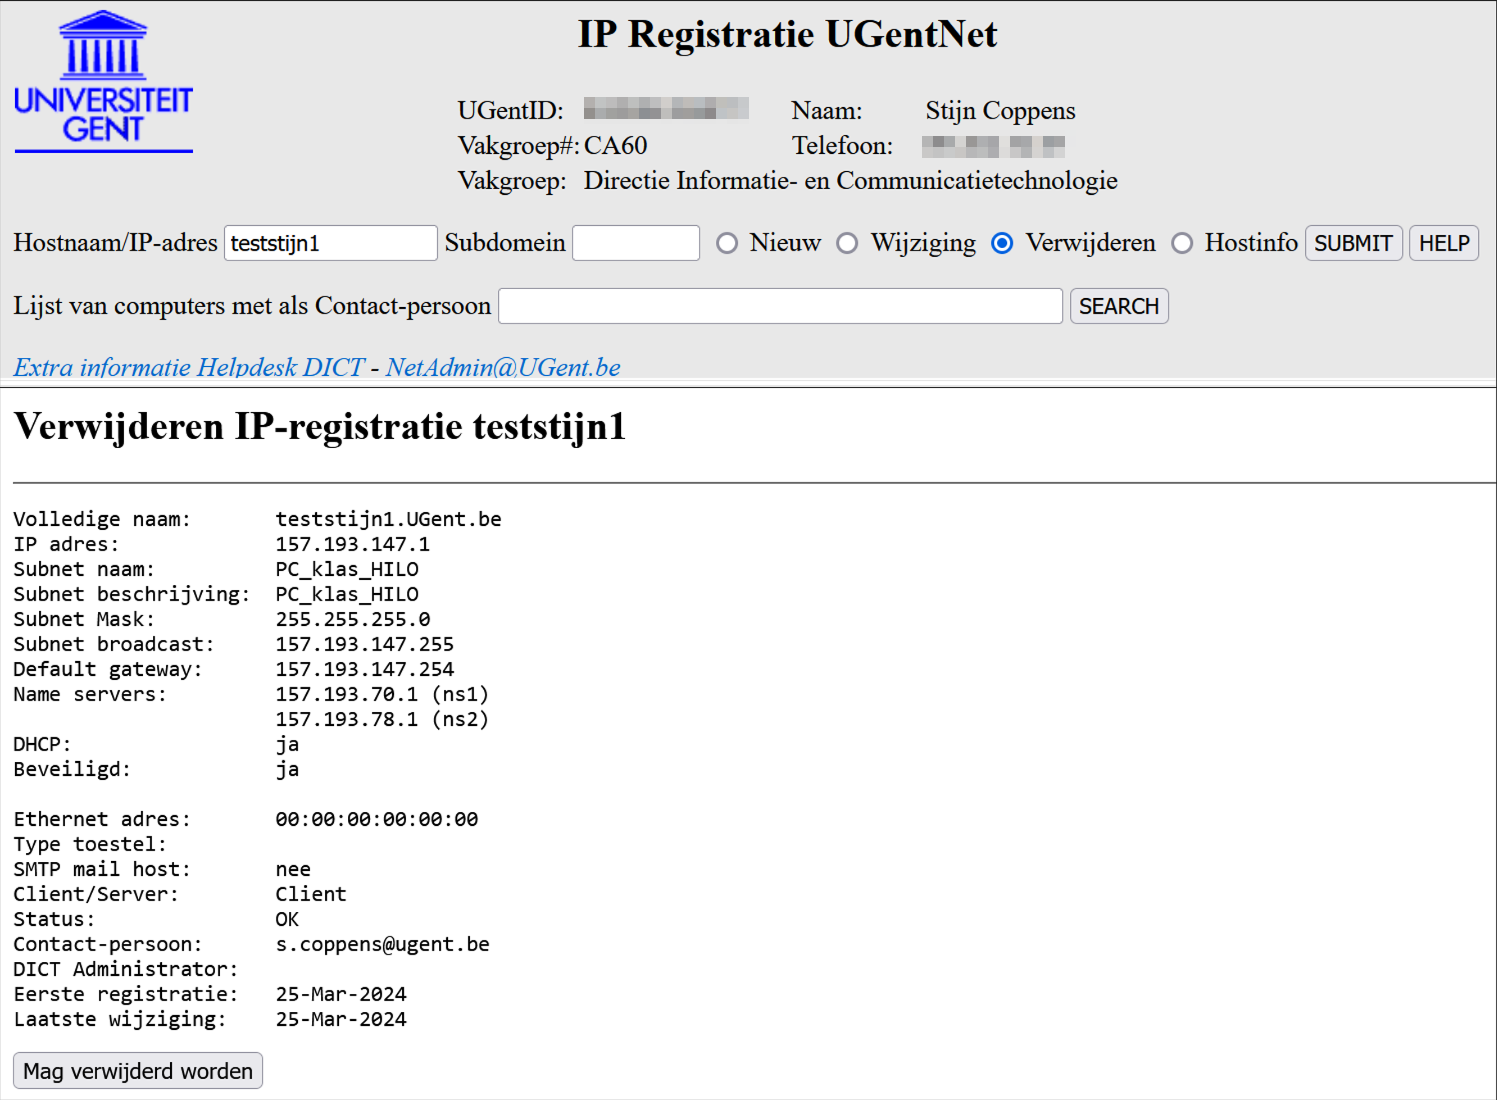
\includegraphics[width=\textwidth]{voorbeeldVerwijderingRegistratieNetadmin.png}
        \caption{Verwijdering IP-registratie}
        \label{fig:formVerwReg}
    \end{subfigure}
    \vskip\baselineskip
    \begin{subfigure}[b]{0.475\textwidth}
        \centering
        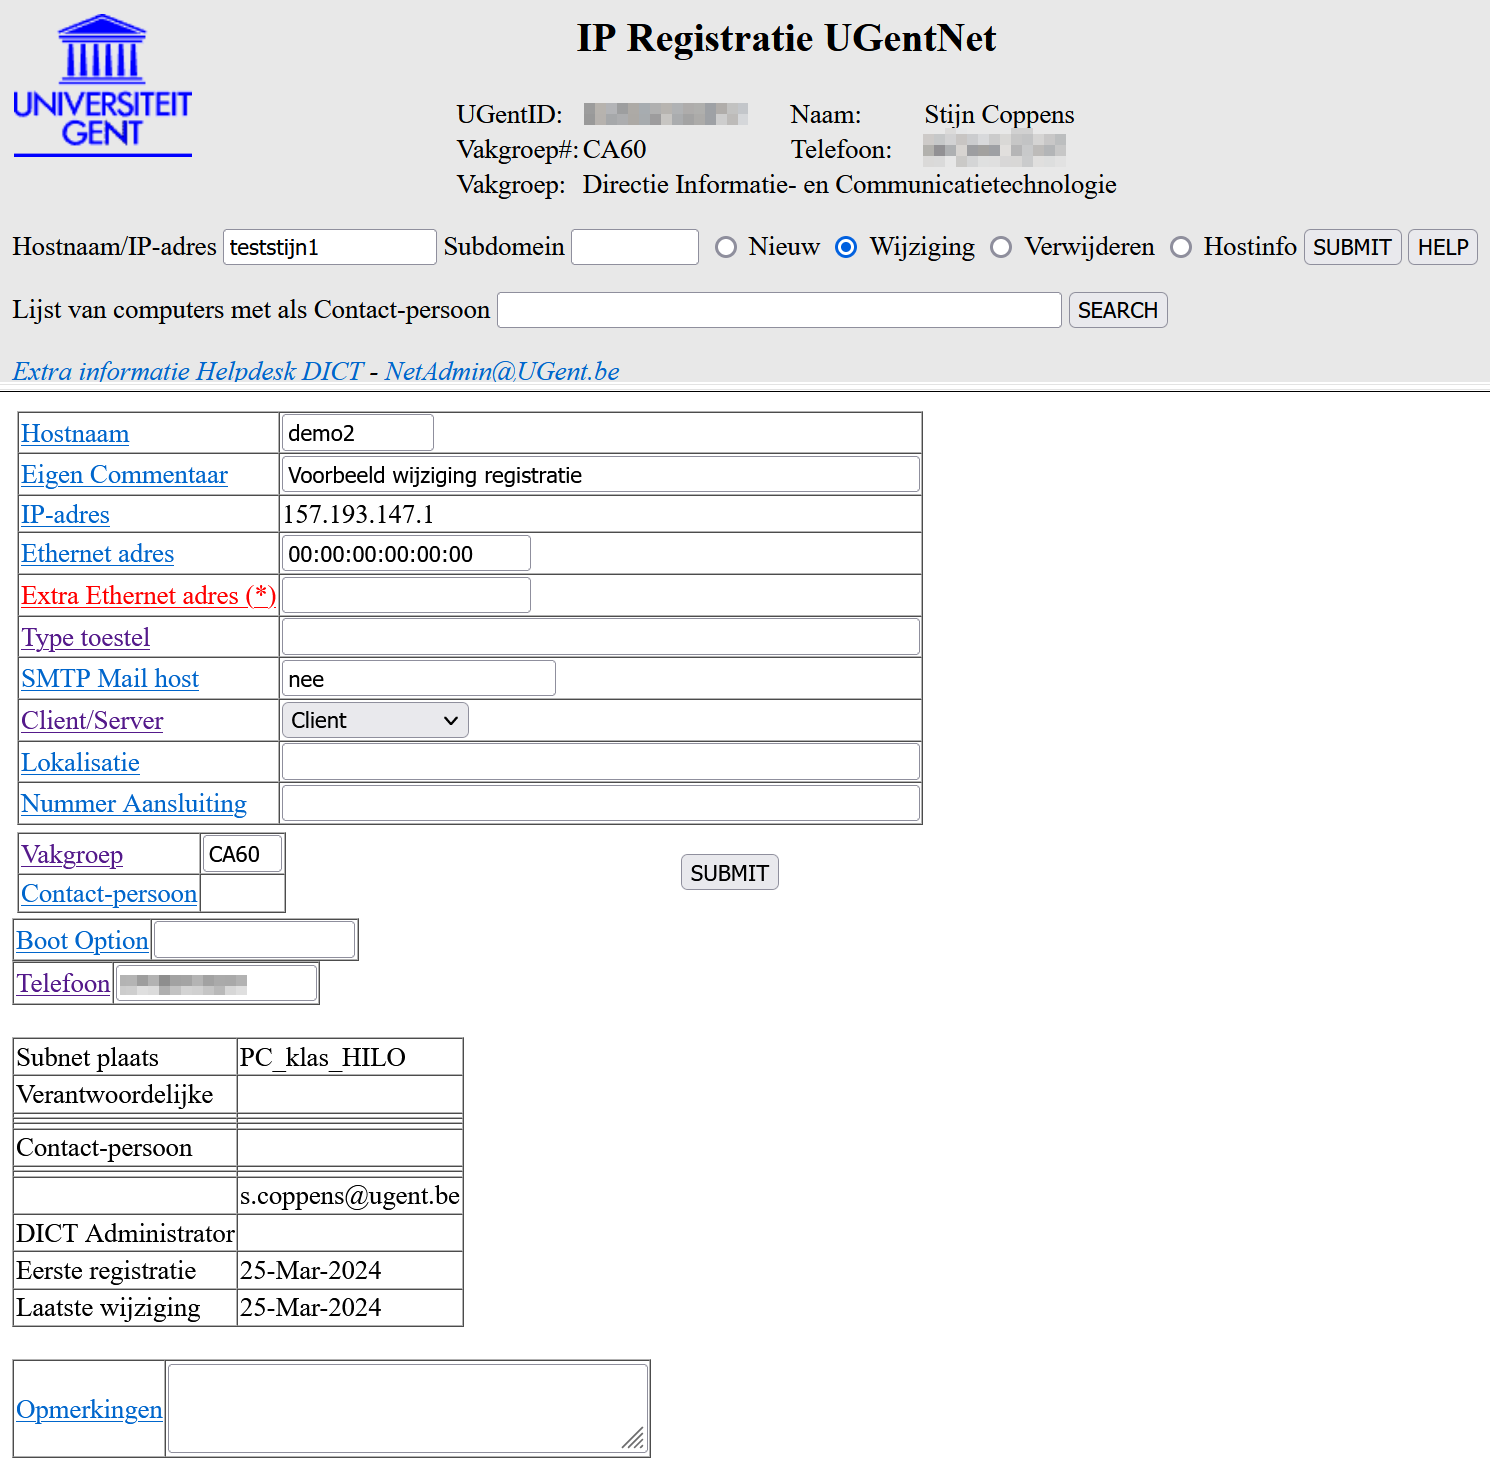
\includegraphics[width=\textwidth]{voorbeeldWijzigingRegistratieNetadmin.png}
        \caption{Formulier wijziging IP-registratie}
        \label{fig:formWijzReg}
    \end{subfigure}
    \hfill
    \begin{subfigure}[b]{0.475\textwidth}        
        \centering
        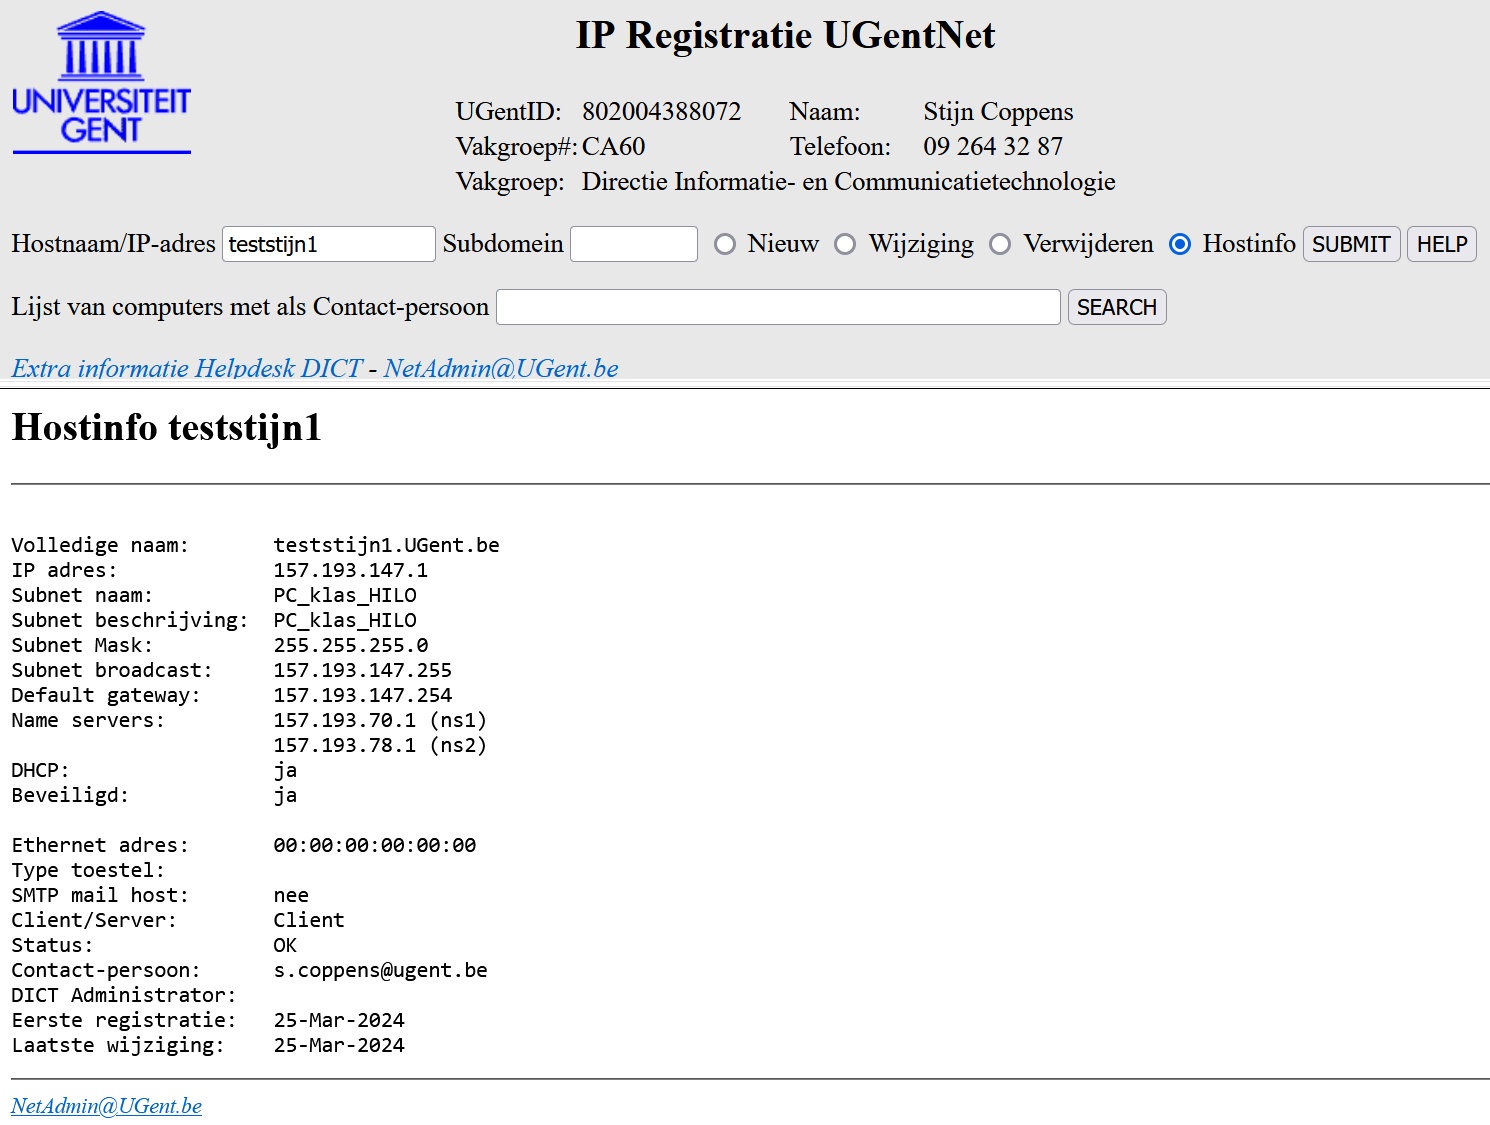
\includegraphics[width=\textwidth]{netadminRaadplegen.png}
        \caption{Raadplegen IP-registratie}
        \label{fig:raadReg}
    \end{subfigure}    
    \caption{Netadmin website IP-registratie}
    \label{fig:netadmin}
\end{figure*}


\subsubsection{Procedure IP registratie voor netwerkbeheerders}
\textcolor{purple}{Nadat de gebruiker op submit klikt zal de backend van de website de ingegeven informatie verwerken en als mail verzenden naar de gedeelde mailbox netadmin@ugent.be. Afbeelding \ref{fig:netadminMail} toont drie mails die een netwerkbeheerder dient te behandelen. 
Elke mail bevat steeds een commando, deze dient de netwerkbeheerder uit te voeren op de daarvoor bestemde server in de folder waarin de subnetbestanden staan. Alle informatie in deze afbeeldingen is op basis van de ingegeven informatie in figuren \ref{fig:netadmin}.}
\textcolor{purple}{
\begin{itemize}
    \item Figuur \ref{fig:nieuwRegMail}: Deze mail geeft alle nodige informatie terug om een nieuwe IP registratie te maken. Het in de mail beschreven commando \textbf{mkh B 147 demonstratie} zal enkele belangrijke taken en controles uitvoeren, waarna de cursor van de beheerder in het eerste vrije adres geplaatst wordt van subnetbestand subnetB147.000. Hierna kan de beheerder alles uit de mail kopiëren beginnende bij \textit{21ddkA} tot en met het einde van de host registratie. Nadat de beheerder het subnetbestand afsluit zal het script nog enkele controles uitvoeren voor het geval er fouten in de registratie staan. Indien de gebruiker in het opmerkingenveld nog informatie heeft geplaatst zoals netwerkpoorten die open moeten staan, DNS Alias records of andere, dient de netwerkbeheerder dit manueel nog aan te vullen in het subnetbestand.
    \item Figuur \ref{fig:wijzigRegMail}: Deze mail bevat alles voor het wijzigen van een bestaande registratie, het commando in deze mail is \textbf{chh B 147 teststijn1 demo2}. Dit heeft een gelijkaardige uitvoeren als bij het aanmaken van een nieuwe registratie, echter zal hier gezocht worden naar de opgegeven host, in dit geval \textit{teststijn1}. Omdat er een tweede hostnaam is opgegeven zal het commando de hostnaam ook wijzigen naar dit tweede hostnaam.
    \item Figuur \ref{fig:verwRegMail}: Deze mail geeft het commando \textbf{rmhost B 147 teststijn1}. Dit commando zal de host in subnet B 147 opzoeken en vervangen door een lege, vrije host. Dit is het enige commando waarbij de netwerkbeheerder niet in het bestand hoeft te gaan om data te plaatsen waardoor deze ook zeer beperkt is in uitvoeringstijd.
\end{itemize}}

\begin{figure}[H]
    \subfloat[Nieuwe IP registratie]{%
        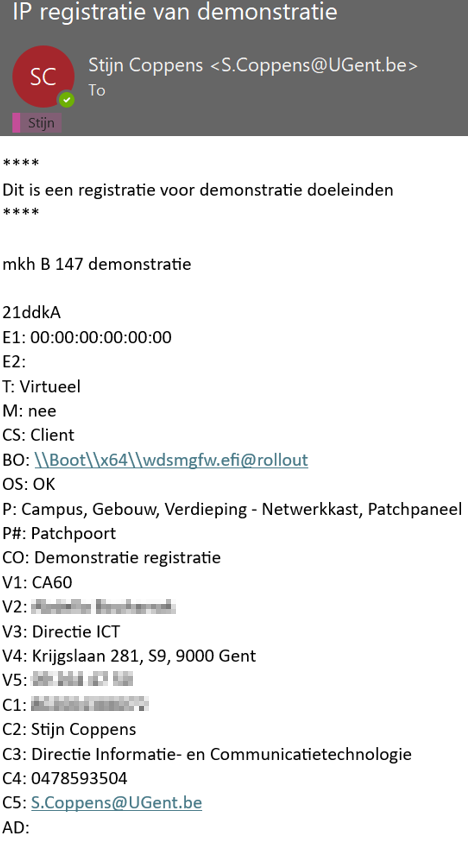
\includegraphics[height=0.4\textheight]{mailNieuweRegistratie.png}
        \label{fig:nieuwRegMail}}
    \hspace*{\fill}
    \subfloat[Wijziging hostnaam IP registratie]{%
        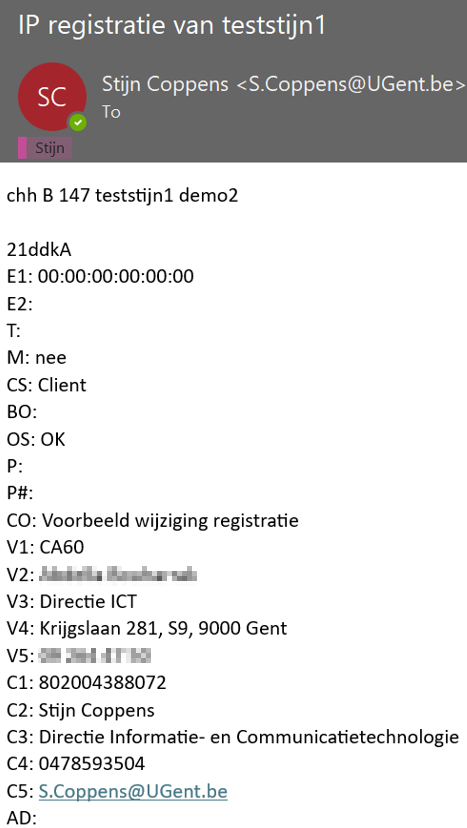
\includegraphics[height=0.4\textheight]{mailWijzigingRegistratie.png}
        \label{fig:wijzigRegMail}}
    \hspace*{\fill}
    \subfloat[Verwijderen IP registratie]{%
        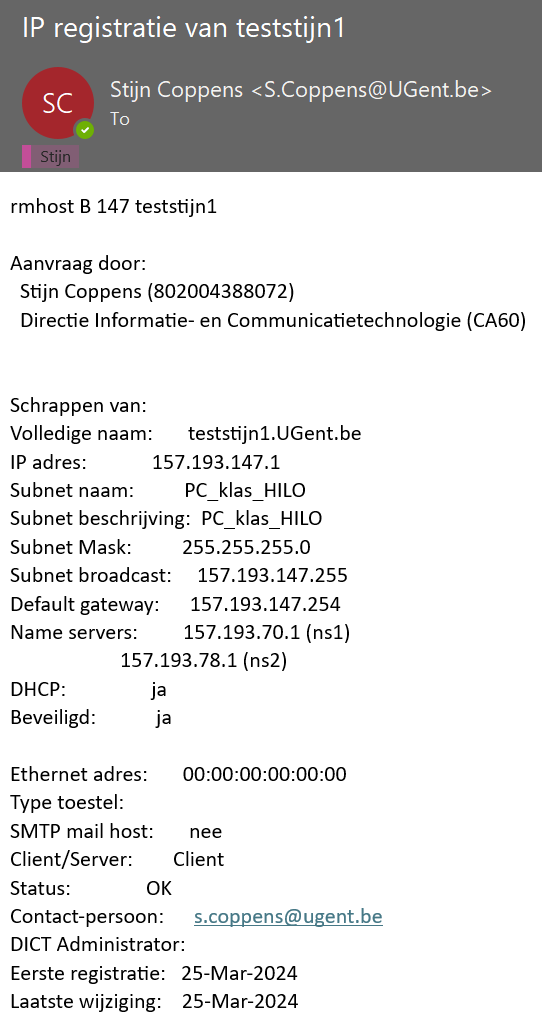
\includegraphics[height=0.4\textheight]{mailVerwijderenRegistratie.png}
        \label{fig:verwRegMail}}
    \caption{mails IP Registratie}
    \label{fig:netadminMail}
\end{figure}

\subsubsection{Aanvullende belangrijke commando's voor subnetbestanden}
\textcolor{purple}{Naast de drie commando's \textbf{mkh}, \textbf{cch} en \textbf{rmhost} voor het verwerken van IP registraties, zijn er nog enkele andere commando's die relevant zijn te vermelden. }
\textcolor{purple}{
\begin{itemize}
    \item Hosts verplaatsen: vb. \textbf{mvh B 147 B 50 teststijn1} zal een host verplaatsen van subnetbestand subnetB147.000 naar subnetB50.000 
    \item Subnetten opkuisen: vb. \textbf{unused B 147 400} geeft alle hosts weer die 400 dagen offline zijn, \textbf{unused\_rmhost B 147 400} geeft alle commando's om diezelfde hosts te verwijderen.
\end{itemize}
}

\textcolor{purple}{Het \textbf{mkh} commando zal steeds laten weten als er geen vrij IP-adressen meer zijn in een subnet. Hier zal de netwerkbeheerder een opkuisactie moeten doen door in te loggen op een andere daarvoor bestemde server, en hier het \textbf{unused B 147 400} te gebruiken. Via een pipeline en \textbf{grep} kan de netwerkbeheerder de lijst van hosts nog verder filteren op basis van bv. jaartal. Zo krijg je een gelijkaardig commando als \textbf{unused B 147 400 | grep -v 202[0-4] | grep -v 201[5-9]}. 
Dit commando zal enkel hosts tonen die niet meer online zijn geweest sinds voor 2015. Eens de netwerkbeheerder tevreden is van het aantal hosts die verwijdert zullen worden, kan die het commando nog eens uitvoeren maar dan met \textbf{unused\_rmhost} in plaats van \textbf{unused}. De output van dit commando zal alle gevraagde rmhost commando's oplijsten die de netwerkbeheerder op de subnetbestanden server kan uitvoeren.}

\textcolor{purple}{Naast deze commando's zijn er ook nog de update-commando's. Pas nadat deze uitgevoerd zijn zullen alle registraties die gemaakt zijn sinds de vorige uitvoering ook effectief van toepassing zijn.}
\textcolor{purple}{
\begin{itemize}
    \item \textbf{update\_all -load}: Dit commando zal alle nodige bestanden maken en actief zetten in de \acrshort{dns}-server.
    \item \textbf{update\_dhcp}: Dit commando doet het nodige voor DHCP
    \item \textbf{update\_hostlst}: Dit commando doet de nodige opruimacties voor subnetbestanden
    \item \textbf{mkacl}: Dit commando overloopt alle aangemaakt ACL's
    \item \textbf{update\_acl\_no\_write}: Dit commando vraagt nog een wachtwoord en zal alle ACL's communiceren met de nodige routers.
\end{itemize}
}
%\begin{figure}[H]
%    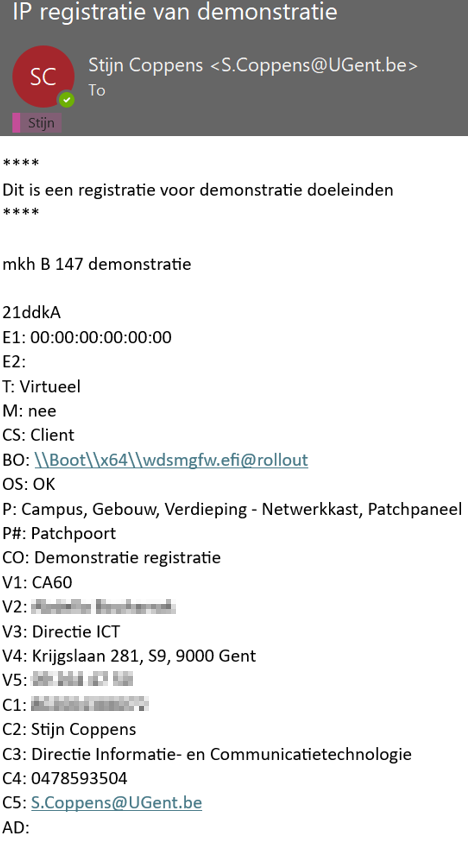
\includegraphics[height=7cm]{mailNieuweRegistratie.png}
%    \caption{Inhoud mail van nieuwe IP-registratie}
%    \label{fig:netadminMail}
%\end{figure}

\subsection{Status migratie subnetbestanden naar EfficientIP}
\lipsum[0-1]
\subsection{Volgende stappen in de migratie}
\lipsum[2-3]

% TODO: Beschrijven wat er reeds gedaan is tot nu toe voor de overstap naar EIP
% TODO: Stappen beschrijven hoe we overgaan naar EIP

